%\part*{Lezione 22/03/2021}
\begin{figure}[h]
    \centering
    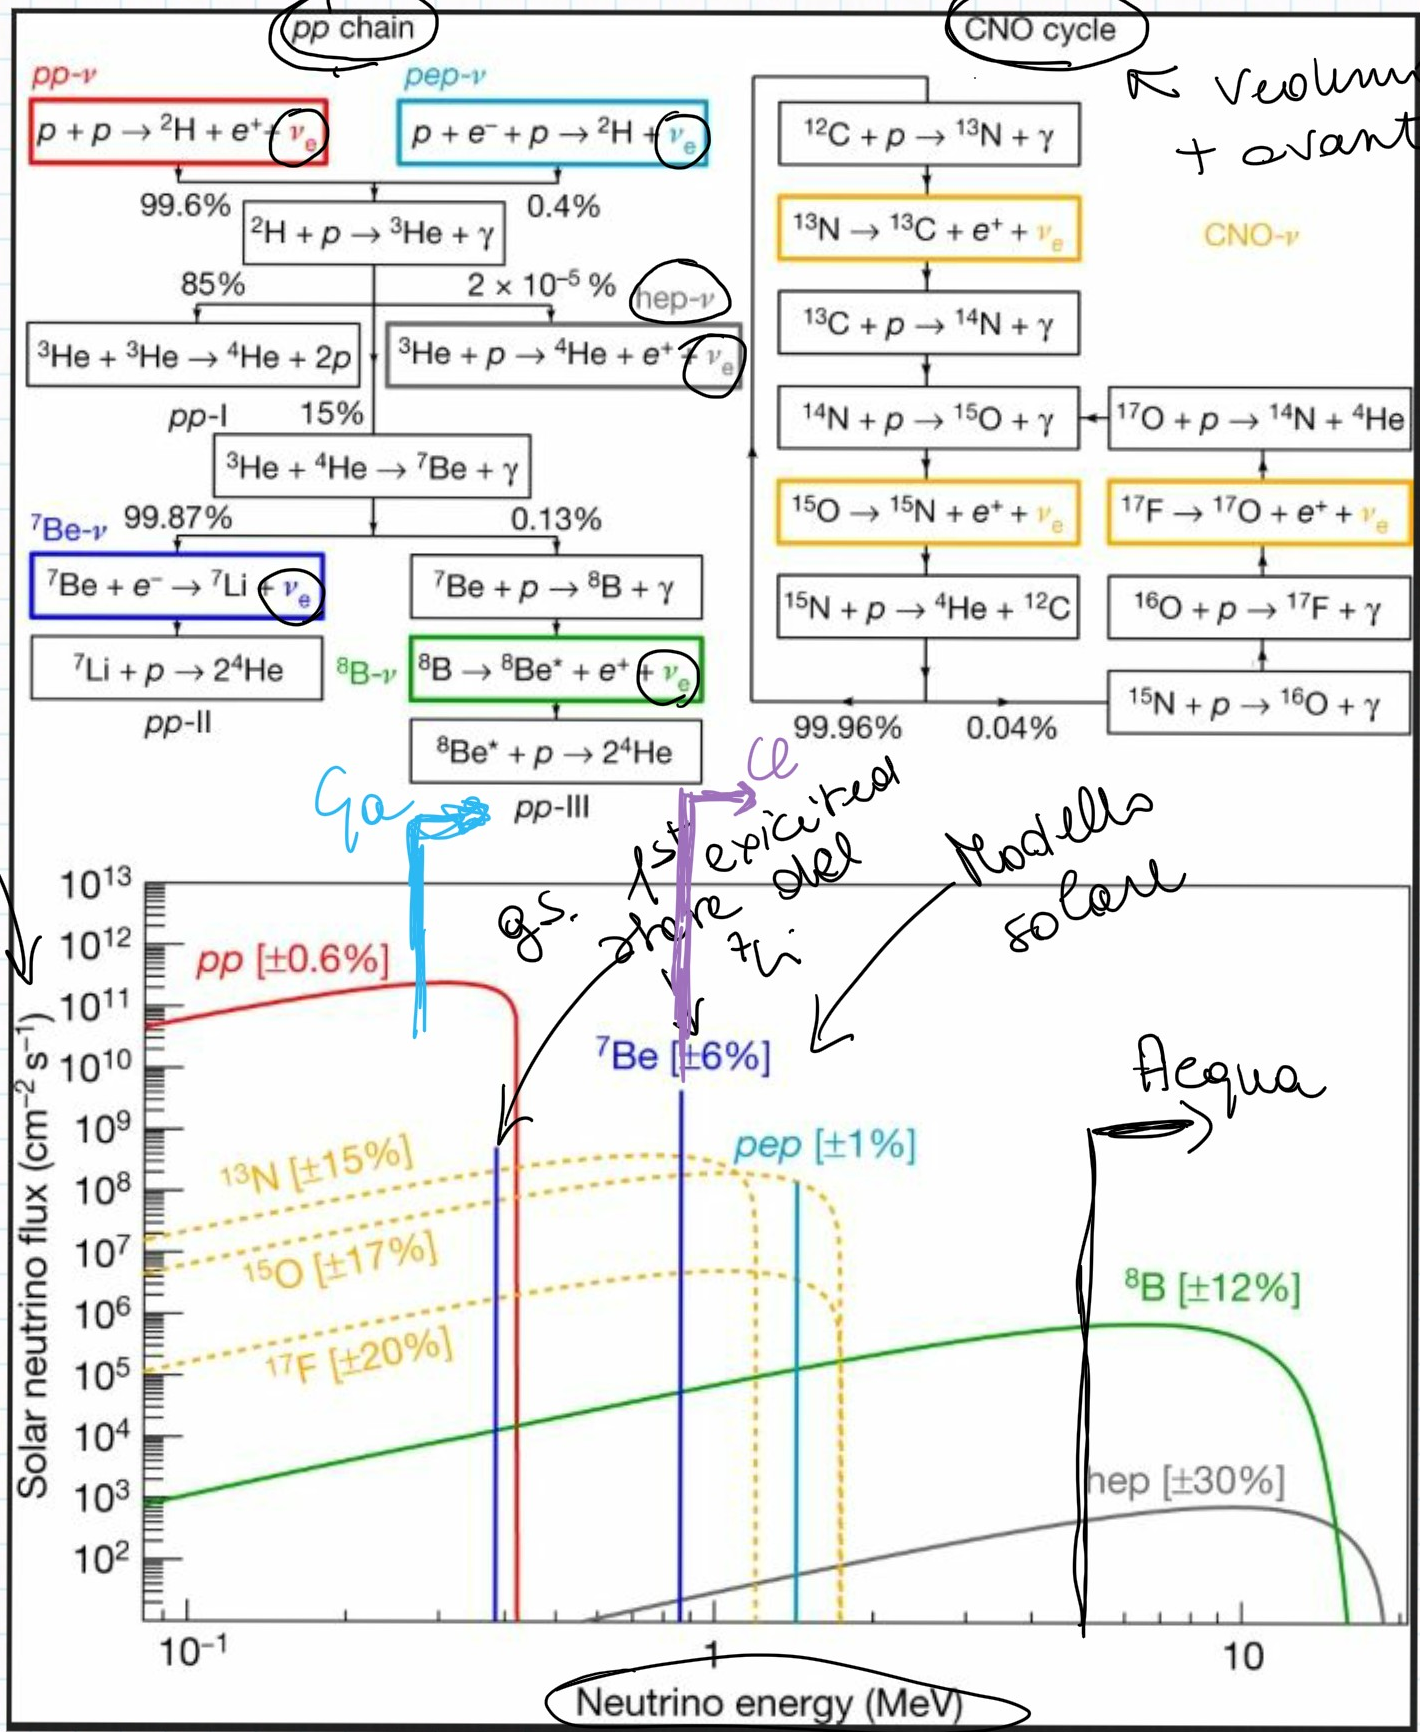
\includegraphics[scale=0.2]{Immagini/0322_neutrini.png}
    \caption[I due processi di produzione dell'elio nel Sole: la catena $pp$ e il biciclo CN-NO. Sotto sono riportati risultati teorici per il vari flussi di neutrini in funzione della loro energia in base alla reazione che li ha prodotti: i rossi, i verdi e i grigi sono uno spettro continuo e il massimo dipende dal fatto che il neutrino è uno di tre corpi; i blu e il turchese sono righe. Ogni flusso ha ovviamente una certa incertezza teorica. La linea viola indica la soglia per l'esperimento di Davis, quella celeste per l'esperimento con il gallio e quella nera per esperimenti con l'acqua. I neutrini del CN-NO hanno tutti uno spettro continuo e sono indicati in giallo.]{I due processi di produzione dell'elio nel Sole: la catena $pp$\index{Catena protone-protone@Catena protone-protone $pp$} e il biciclo CN-NO\index{Ciclo CNNO@Ciclo CN-NO}\footnotemark. Sotto sono riportati risultati teorici per il vari flussi di neutrini in funzione della loro energia in base alla reazione che li ha prodotti: i rossi, i verdi e i grigi sono uno spettro continuo e il massimo dipende dal fatto che il neutrino è uno di tre corpi; i blu e il turchese sono righe. Ogni flusso ha ovviamente una certa incertezza teorica. La linea viola indica la soglia per l'esperimento di Davis, quella celeste per l'esperimento con il gallio e quella nera per esperimenti con l'acqua. I neutrini del CN-NO hanno tutti uno spettro continuo e sono indicati in giallo.}
    \label{0322_nu}
\end{figure}
\footnotetext[5]{Si veda la sezione \secrif{sec-CNNO}.}
\section{Il problema dei neutrini solari}\label{0322-sec-nu}
Come anticipato precedentemente, i neutrini sono i miglior candidati per la verifica sperimentale della nucleosintesi; il primo esperimento di verifica fu fatto da Richard Davis\esperimento{esperimento di Davis} nel 1960 e gli valse il premio Nobel: egli ebbe l'idea di studiare in una miniera del Sud Dakota (detta \textit{Homestake}) la reazione
$$\ce{^{37}Cl} + \nu_e \to \ce{^{37}Ar} + e^-$$
poiché attraverso analisi chimica è possibile contare Ar estratto ed essendo nel sottosuolo l'effetto dei raggi cosmici è attenuato; tuttavia, è necessario avere Cl purissimo. L'esperimento funzionò, i neutrini furono osservati, ma dal momento che la reazione ha una certa energia di soglia ($E_{th}\sim 1$ MeV) gli unici neutrini visibili furono quelli della $pep$, del $\ce{^8B}$ e della $hep$ che come mostrato in Figura \ref{0322_nu} sono i meno numerosi. Il problema principale, però, fu il fatto che il numero di neutrini osservati era circa la metà di quelli previsti.\\
Inizialmente si imputò questa discrepanza alla natura dell'esperimento per cui ne seguirono altri con reazioni differenti, uno di questi fu GALLEX\esperimento{GALLEX} tra il 1991  il 1997 al Gransasso:
$$\ce{^{71}Ga + \nu_e \to \ce{^{71}Ge}} +e^-$$
in questo caso l'energia di soglia è $E_{th}\simeq 233.2$ keV (la linea celeste in Figura \ref{0322_nu}), quindi vedo molti più neutrini. Il $\ce{^{71}Ge}$ si estrae attraverso la molecola di germano $\ce{^{71}GeH_4}$ e dato che il tempo di dimezzamento del $\ce{^{71}Ge}$ è di circa $11.43$ giorni i neutrini vengono contati dal numero di decadimenti che si osservano. Nonostante i cambiamenti fatti all'apparato sperimentale, ottennero lo stesso risultato. Furono condotti allora esperimenti con rivelatori \cherenkov{} ad acqua\esperimento{esperimento con acqua}:
$$\nu_e + e^- \to \nu_e + e^- \quad \text{Riculo} \to \text{luce \cherenkov}$$
Il vantaggio della luce \cherenkov{} è che è direzionale quindi era possibile determinare con precisione se i neutrini venissero dal Sole; lo svantaggio è che oltre ad avere bisogno di molta acqua purissima gli eventi sono pochi, perché l'elettrone per emettere deve superare una certa soglia e questo impone che il neutrino abbia energia alta (la soglia nera in Figura \ref{0322_nu}), per cui si osservano solo quelli del $\ce{^8B}$ e della $hep$. Inoltre, ogni tipo di neutrino può fare tale scattering: i $\nu_\tau$ e i $\nu_\mu$ per esempio possono scambiare solo un bosone che sia neutro, quindi, $Z^0$, mentre i $\nu_e$ oltre a $Z^0$ dato che $\nu_e\to e^-$ o $e^-\to \nu_e$ possono mediare l'interazione anche tramite i bosoni $W^\pm$. In generale non c'è modo di distinguere un processo dall'altro, ma dal momento che $m_W\ll m_Z$ questa interazione è molto più probabile (quindi $\nu_e$ in maggior numero).
\begin{figure}[h]
    \centering
    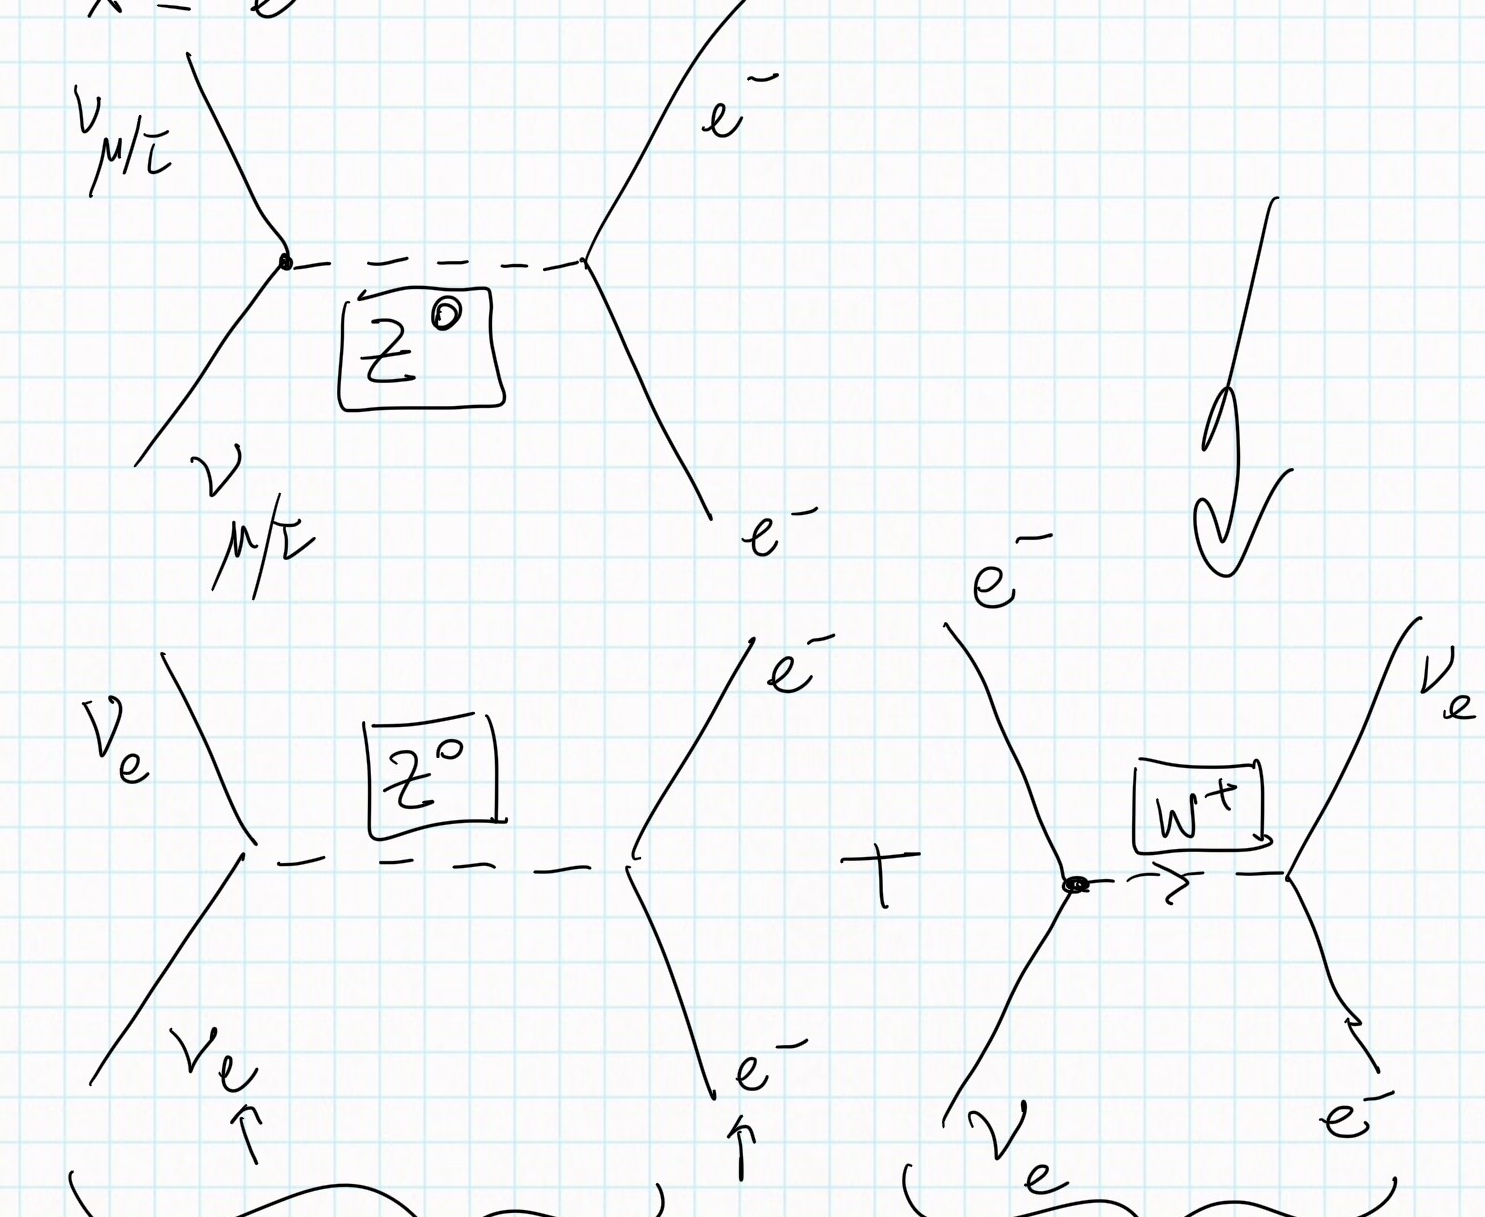
\includegraphics[scale=0.2]{Immagini/0322_Scambio.png}
    \caption{Rappresentazione schematica dell'interazione nello scattering.}
    \label{0322_scambio}
\end{figure}
\noindent Passiamo ora alla descrizione\footnote{Le immagini e i dati sono raccolti nelle \textit{slide} \texttt{Neutrino\_flux\_exp.pdf}.} di 3 esperimenti di questo tipo:
\begin{itemize}
    \item \textbf{Super-Kamiokande} (SK)\esperimento{Super-Kamiokande}: dal nome della miniera Kamioka in Giappone nella quale è situato è il successore del precedente Kamiokande. Contiene una cisterna di $50,000$ tonnellate di acqua costellata di fotomoltiplicatori (maggiormente sensibili ai $\nu_e$) che ne coprono l'intera superficie (circa $11,200$). \\
    Potendo acquisire risultati sia di giorno che di notte, SK osservò una differenza nel numero di neutrini nei due momenti del giorno, in particolare $\#\nu_{notte}<\#\nu_{diurno}$. Per la prima volta però si riesce a dare una spiegazione di queste fluttuazioni: assumendo, infatti, che $m_\nu\not = 0$ si può dimostrare che lo stato di neutrino di interazione debole (quindi di un certo \textit{sapore}) può essere descritto come sovrapposizione di due stati di massa differente %secondo un certo operatore di massa
    , ovvero:
    \begin{displaymath}
    \begin{aligned}
    \st{\nu_e} &= \alpha\, \st{\nu_1} + \beta\, \st{\nu_2}\\
    \st{\nu_\mu} &= \alpha'\, \st{\nu_1} + \beta'\, \st{\nu_2}
    \end{aligned}
    \end{displaymath}
    Lo stato del neutrino di interazione quindi oscilla\index{oscillazione di sapore dei neutrini} $\st{\nu_e}\simeq k \st{\nu_\mu}$ con una probabilità che dipende dalla distanza percorsa prima dell'osservazione e questo spiega la discrepanza con il numero di neutrini previsti dalla teoria. Tuttavia, SK non poté verificarlo perché nel 2001\index{incidente al Super-Kamiokande} durante la manutenzione per la quale viene svuotata la cisterna non si accorsero che un fotomoltiplicatore si era leggermente incrinato e al successivo riempimento, quando il livello era circa a metà, questo fotomoltiplicatore si è rotto; il vuoto al suo interno ha risucchiato l'acqua producendo un'onda d'urto che ha innescato una reazione a catena e ha causando la rottura di 500 fotomoltiplicatori.\\
    Dopo l'incidente i giapponesi iniziarono repentinamente le riparazioni, ma ormai era stato già avviato un altro esperimento in Canada per la verifica della teoria.
    \item \textbf{Sudbury Neutrino Observatory} (SNO)\esperimento{Sudbury Neutrino Observatory}: esperimento con rivelatore \cherenkov{} situato nella miniera Creighton in Canada, sfruttò l'acqua pesante $\ce{^2H_2O}$ invece della semplice $ce{H_2O}$, questo perché oltre allo scattering elastico era possibile anche la reazione\footnote{Si tratta di una $pep$ \vir{al contrario}} $\nu_e + \ce{^2H} \to p+e^-+p$; questa può avvenire solo con $\nu_e$ e si distingue da quella dello scattering dalla luce \cherenkov{} prodotta. Si noti, però, che è anche possibile:
    $\nu + \ce{^2H} \to \nu + p +n$ ovvero scattering elastico. Per tenerne traccia, furono messe delle impurità di $\ce{^{35}Cl}$ così che $\ce{^{35}Cl}+n\to \ce{^{36}Cl +\gamma}$, identificabile quindi dai fotoni prodotti. Fu allora possibile contare sia il numero di neutrini elettronici che quello di neutrini generici e si ottenne l'evidenza di accordo con il valore predetto dalla teoria: non era quindi il modello solare a dover essere rivisto, ma quello standard.
    \item \textbf{Borexino}\esperimento{Borexino}: in ultima battuta diamo uno sguardo anche al contributo italiano nell'ambito di tale ricerca. In quel periodo infatti al Gransasso era stato sistemato un esperimento che si componeva di uno scintillatore\index{scintillatore} in una camera circondata da fotomoltiplicatori. Il vantaggio era quello di avere una soglia per la reazione molto bassa e questo permise a Borexino di verificare che nel Sole erano presenti anche le reazioni $pp$, $\ce{^7Be}$ e $pep$, come mostrato in Figura \ref{0322_risultati}.\\
    \noindent Una piccola nota dolente: Borexino sarebbe stato capace di verificare l'oscillazione dei neutrini prima dell'esperimento canadese, tuttavia la burocrazia italiana ha ritardato enormemente l'arrivo dei fondi.
    \begin{figure}[ph]
        \centering
        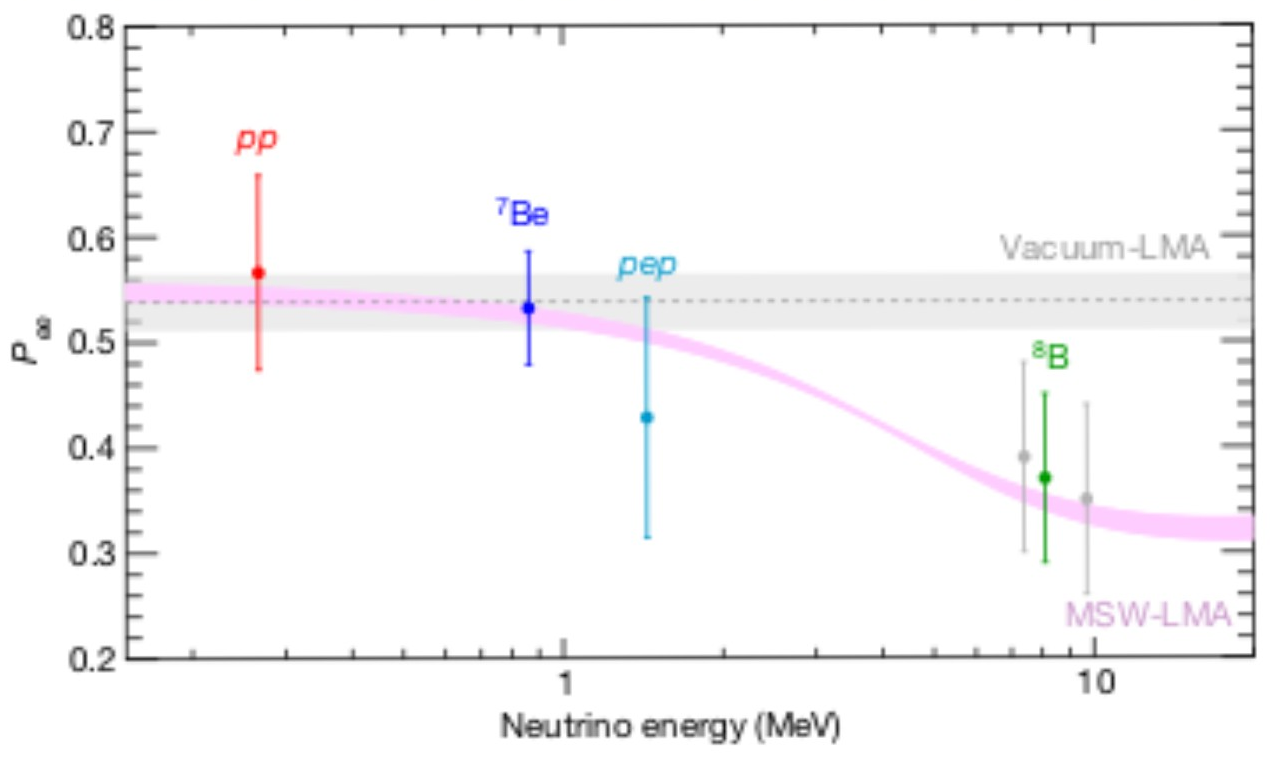
\includegraphics[scale=0.2]{Immagini/0322_energianu.png}
        \caption{Probabilità di sopravvivenza del neutrino in funzione della sua energia. I punti sono i risultati ottenuti da Borexino, in rosa la predizione teorica e in grigio il modello con parametri di oscillazione dati dai risultati di SNO.}
        \label{0322_risultati}
    \end{figure}
    \begin{figure}[p!h]
        \centering
        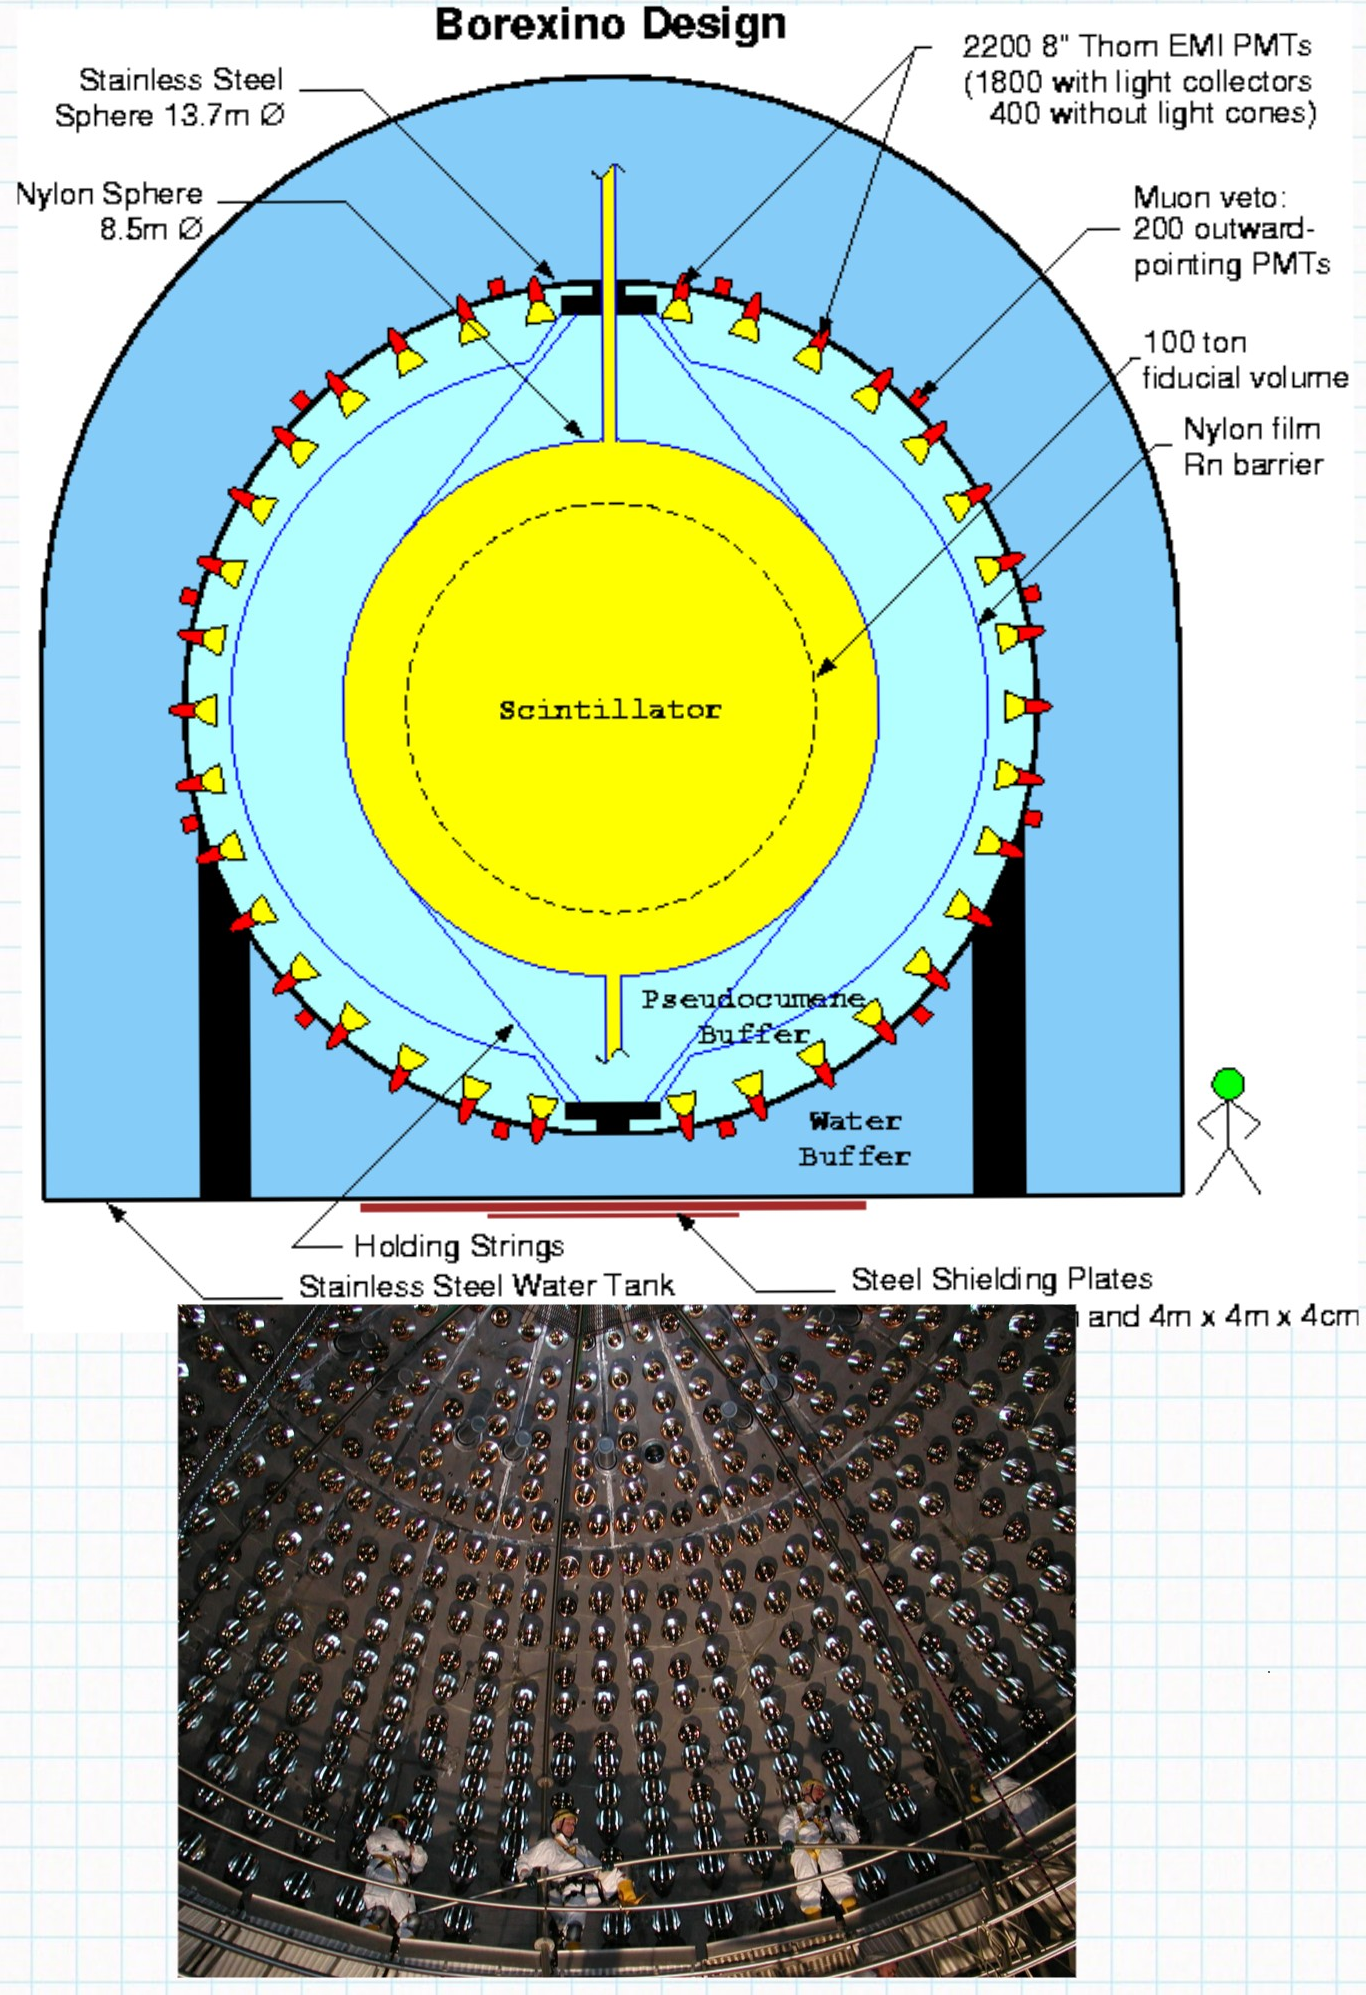
\includegraphics[scale=0.2]{Immagini/0322_borexino.png}
        \caption{Schema e foto dell'esperimento Borexino.}
        \label{0322_box}
    \end{figure}
\end{itemize}

\newpage

\section{Elementi di analisi}
Introduciamo adesso alcuni elementi essenziali per l'analisi nucleare, che utilizzeremo successivamente nello studio della catena $pp$.

\subsection{Fattore Astrofisico}\label{sec-SE}
Consideriamo una generica reazione con particelle (proiettili) che incidono su nuclei (bersagli):
$$a+X\to b+Y$$
Dall'analisi dimensionale abbiamo per la sezione d'urto:
$$\sigma[L^2] = \frac{\# \text{reazioni}/\text{nucleo X}/\text{unità di tempo}}{\underbrace{\# \text{proiettili}/L^2/\text{unità di tempo}}_\text{flusso particelle incidenti}}$$
%\footnote{Nell'espressione abbiamo chiamato \textit{rate} il numeratore; in realtà, il \textit{rate} è in unità di volume e non di nucleo $X$.}
Cerchiamo di costruire l'espressione per il \textit{reaction-rate} $r$\index{reaction-rate@\textit{reaction-rate} $r$}: se $N_a$ è la densità numerica dei proiettili, $\vec{v}$ la loro velocità di volo e $N_X$ la densità numerica dei bersagli allora si ha $r = N_a N_X\, \sigma v$; in generale però potremmo avere $a=X$ e non potendo distinguere tra i due con l'espressione precedente si otterrebbe il doppio del \textit{rate} effettivo, per cui: 
$$r = \frac{N_a N_X}{1+\delta_{aX}}\: \mean{\sigma(\vec{v})\, v}$$
dove abbiamo mediato sulla distribuzione in velocità, che nel caso stellare è una Maxwelliana $\phi(v)$, poiché in generale non tutti i proiettili avranno velocità $\vec{v}$. Procedendo con il calcolo:
\begin{displaymath}
\begin{aligned}
\mean{\sigma(\vec{v})\, v} &= \int_0^\infty \sigma \, v \: \phi(v) dv = \\
&= \int_0^\infty \sigma \, v \: 4\pi \ppc{\frac{\mu}{2\pi kT}}^{3/2} \exp{\ppc{-\frac{\mu v^2}{2kT}}} v^2 dv = \qquad \text{sostituendo } E= \frac{1}{2}\mu v^2\\
&= 4\pi \ppc{\frac{\mu}{2\pi kT}}^{3/2} \int_0^\infty \frac{1}{\mu^2} 2E\, \sigma(E) \, e^{-E/kT} \: dE =\\
&= \sqrt{\frac{8}{\pi \mu}} \ppc{\frac{1}{kT}}^{3/2} \, \int_0^\infty \sigma(E) \, e^{-E/kT} \: dE
\end{aligned}
\end{displaymath}
La dipendenza di $\sigma$ da $E$ dipende principalmente da tre fattori:
\begin{enumerate}
    \item La probabilità di attraversamento della barriera Coulombiana.
    \item La probabilità di avere un'interazione.
    \item La prossimità a una risonanza nucleare.\index{risonanza nucleare}
\end{enumerate}
Tutti e tre infatti dipendono dall'energia. Studiamo prima le reazioni non-risonanti: per il contributo 2. dalla meccanica quantistica sappiamo che la probabilità di interazione è proporzionale a\footnote{$\pi\lambda_{DB}^2$ non è altro che la sezione d'urto.} $\pi \lambda^2_{DB}\sim p^{-2} \sim E^{-1}$\index{lunghezza d'onda di De Broglie@lunghezza d'onda di De Broglie $\lambda_{DB}$}; per il contributo 1. l'espressione è un po' più complessa, ma nel Sole ho tutte particelle cariche quindi:
$$V = \frac{Z_1 Z_2 e^2}{r} \simeq 1.44 \, \frac{Z_1Z_2}{r[\mbox{fm}]} [\mbox{MeV}] \underset{\text{per }pp}{\sim} 1.44\unit{MeV}$$
L'energia di agitazione termica media $\mean{E}\sim kT \sim 9\cdot\ord{-8} \, T[\mbox{K}]\,[\mbox{keV}]$ per la temperatura interna del Sole ($T\sim 1.5\cdot\ord{7}$ K) è dell'ordine del keV, quindi trascurabile rispetto alla barriera. Valutiamo allora la probabilità di attraversamento per effetto tunnel\index{effetto tunnel}\footnote{Per il calcolo guarda \complrif{compl-tunnel}.}:\label{sec-tunnel}
\begin{displaymath}
\begin{aligned}
P &\sim \exp{\PPc{-2\pi \frac{Z_1Z_2 e^2}{\hbar v}}} =\\
&= \exp{\PPc{-2\pi \frac{Z_1Z_2 e^2}{\hbar}\, \sqrt{\frac{\mu}{2E}}}} =\\
&= \exp{\PPc{-\sqrt{2\mu}\pi\, \frac{Z_1Z_2 e^2}{\hbar \sqrt{E}}}} 
\end{aligned}
\end{displaymath}
detto \textbf{fattore di penetrazione di Gamow}\index{fattore di penetrazione di Gamow}. Per quanto riguarda i vari contributi nucleari possiamo raccoglierli tutti in un fattore $S(E)$ che chiamiamo \textbf{fattore astrofisico}\index{fattore astrofisico@fattore astrofisico $S(E)$}; abbiamo allora:
$$\sigma (E) = \frac{1}{E}\,\exp{\PPc{-\sqrt{2\mu}\pi\, \frac{Z_1Z_2 e^2}{\hbar \sqrt{E}}}}\, S(E)$$
\noindent A titolo di esempio riportiamo l'andamento di $\sigma(E)$ per la reazione $\ce{^{12}C}+p\to \ce{^{13}N}+\gamma$ in Figura \ref{0322_cross}. Si osserva una risonanza per circa $0.5$ MeV e la drastica pendenza della sezione d'urto sotto $0.3$ MeV (dovuta al fattore di Gamow); in rosso è segnato il range di energie di interesse astrofisico.
\begin{figure}[!h]
    \centering
    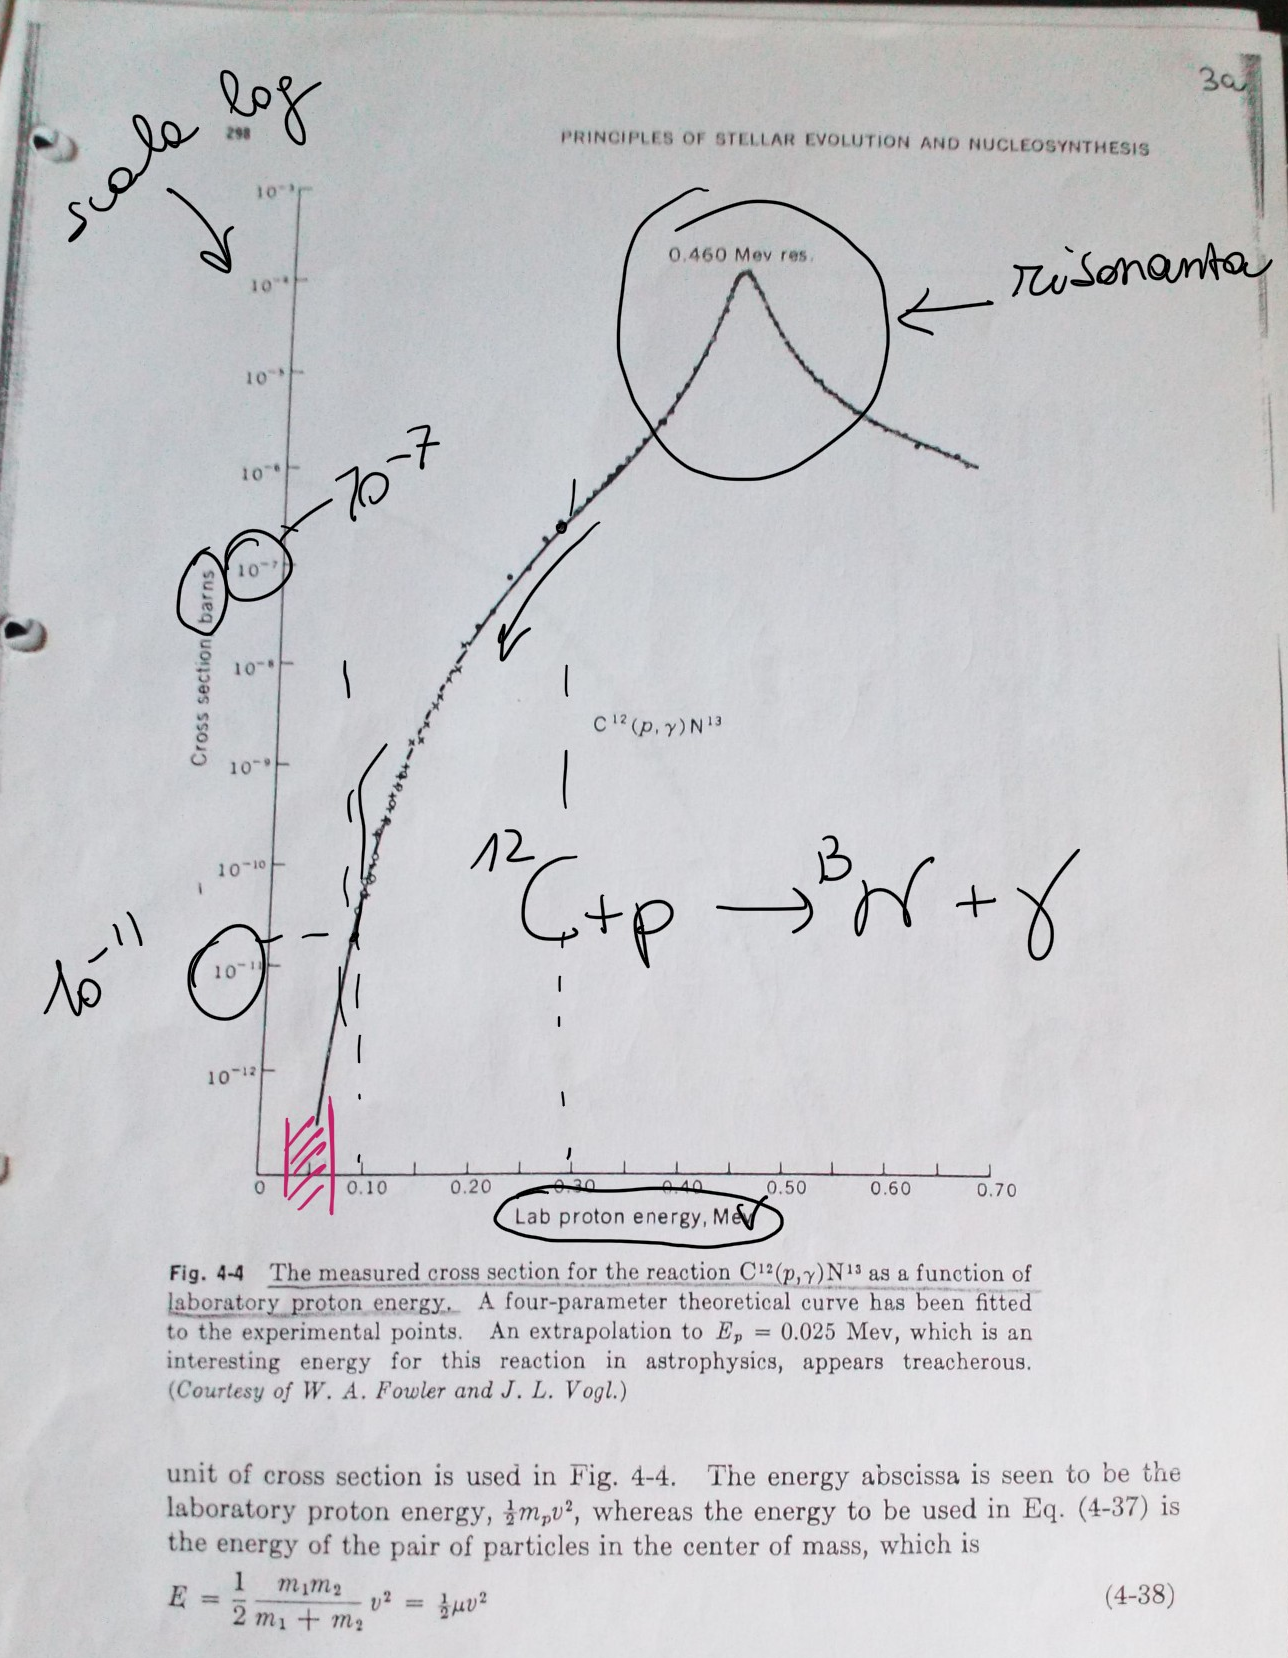
\includegraphics[scale=0.2]{Immagini/0322_crosssection.png}
    \caption{Leggere la didascalia. In rosso il range di energie di interesse astrofisico.}
    \label{0322_cross}
\end{figure}\\
\noindent Dall'espressione per la sezione d'urto possiamo invertire così da ottenere l'andamento del fattore astrofisico $S(E) = E \sigma(E)\exp(\dots)$ come mostrato in Figura \ref{0322_fatastr}. Si nota che in questo caso l'andamento per basse energie è più \vir{dolce}.

\begin{figure}[h]
    \centering
    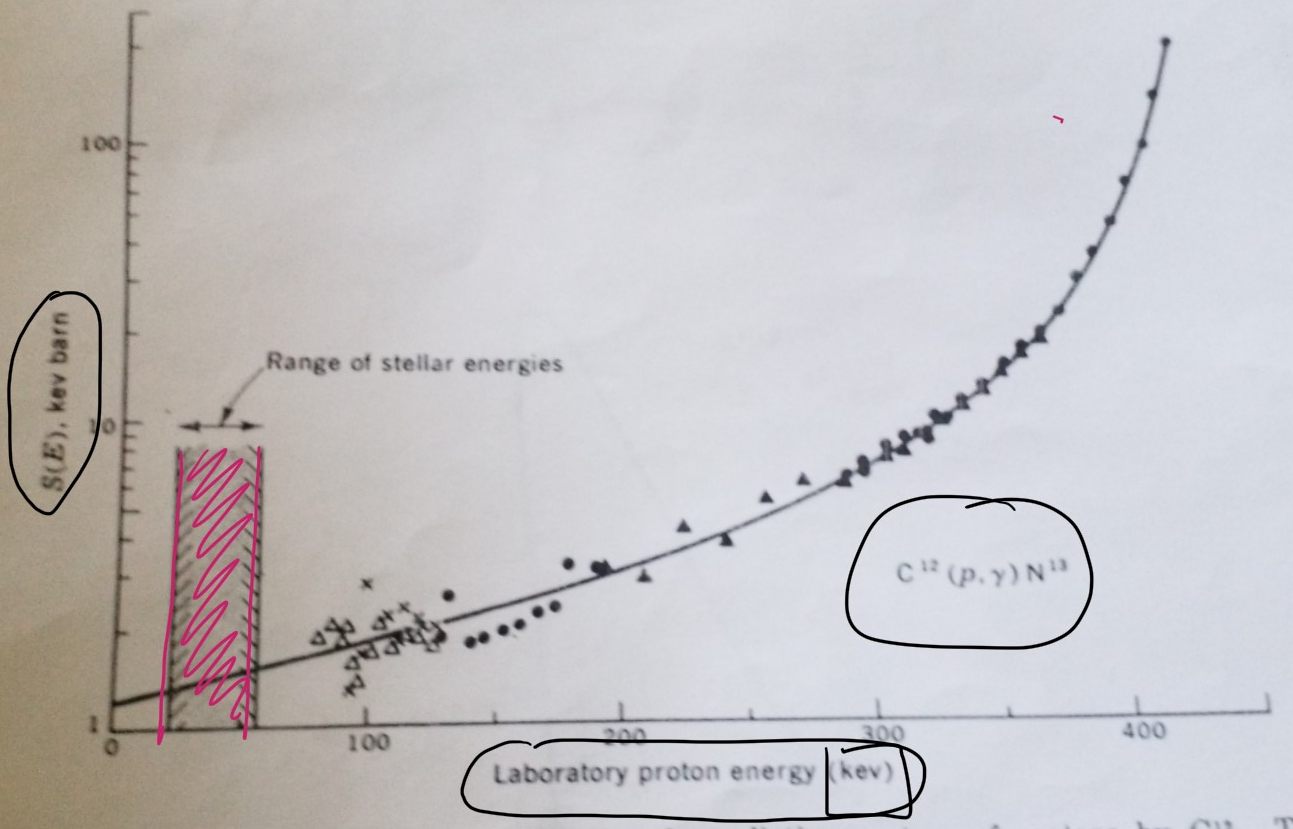
\includegraphics[scale=0.3]{Immagini/0322_fattoreastr.png}
    \caption{Andamento del fattore astrofisico per la reazione precedente.}
    \label{0322_fatastr}
\end{figure}
